% Chapte 9
\chapter{Advertisement enhancement} % Main chapter title

\label{Chapter9} % For referencing the chapter elsewhere, use \ref{Chapter1} 
\newpage






\section{Introduction}

The very first phase to get passers-by engaged with the display is the getting their attention. In previous experiment during the course of five days, only \%12 of the entire of passers-by were attracted and engaged, there could be many reasons, (1) the passers-by could not see their silhouette until got very close to the display and camera and by that time the passers-by might have turned his/her face from the display without looking to their silhouette, (2) Passing by the screen happens within a short amount of second and that is not enough for passers-by to understand interactivity quickly, if the screen is large and placed in front it takes about 1.2 to understand interactivity \cite{LookingGlass}, but my display was in sideways and small, so i assume that it takes longer than 1.2 seconds to understand interactivity and by that time the passers-by has passed the screen, (3) from the observations made during three weeks, most passers-by turned their faces toward the table, which was located in front of the display, and walked around the table to look for books and even did not see the display.

In existing real scenarios like in the tourist information center, where I conducted the study, the display was placed at sideways, and there was no other way to change the location of display to be more in front of passers-by to have more attention of people, therefor I took this real time scenario and proposed an extended version of attracting attention design to enhance the attention level of passers-by, who were far or at corner of display and still could be tracked by display. The chapter also discusses on the study design and evaluation of this technique and meanwhile compares this technique with the previous technique to see the effectiveness and advantages.


\section{Enhanced attracting attention}
The change in the new version was to extend the tracking area about 180 degree around display, this would over come the issues pointed before, because when passers-by walk from the sides the camera can track them and the application can project their silhouette, by doing this there will be enough time for passers-by to get attracted while coming toward display. 

To achieve this, three Kinect cameras were integrated in the sides and in the center of the display and the tracked passers-by silhouette images were stacked together and shown on the display, a person passing from the side could see his self at the side of the screen and when moving to the middle of the screen the application could smoothly transition the person from side camera to the center camera by having the same silhouette color, physically the cameras were positioned side-by-side, therefor there was a small gap for each camera range, which was not perceivable by passers-by. Kinect cameras were tracking individually the users, so the user in the first Kinect was not the same user in the second Kinect and as a result Kinect would give different colors to the same user while passing by each camera, therefor only one color was chosen for all users so that they do not see the shift from camera to other. 

See the diagram bellow that shows the physical setup including Kinect camera and their ranges, the diagram shows three different person standing at each camera range and the system has mapped their silhouette representation that all have the same color on the screen sections relative to their distance to the screen.


\begin{figure}[H]
    \centering
    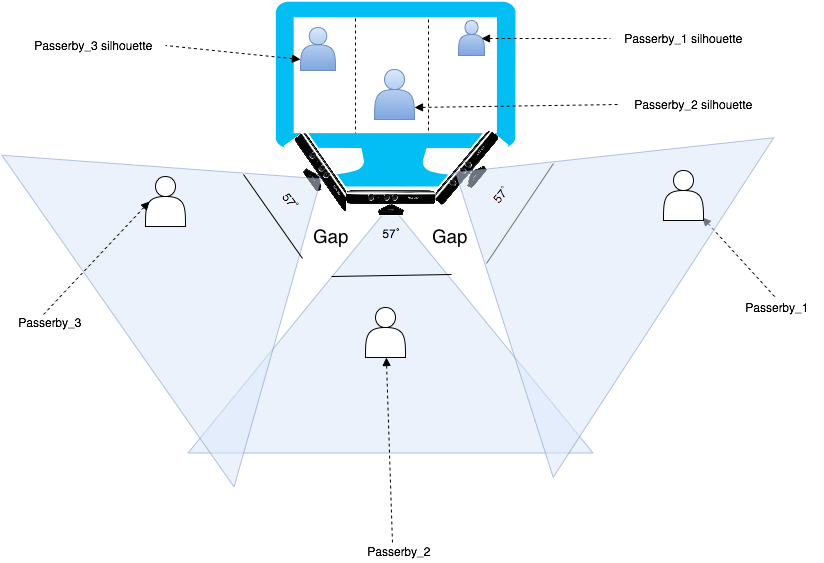
\includegraphics[width=0.9\textwidth,height=8cm]{Figures/9/Kinect_Extended}
    \caption{Attracting attention extended version.}%
    \label{fig:KinectExtended}%
\end{figure}


\section{Interaction design}
The interaction design for the extended version is completely the same as the body interaction design that was introduced in chapter 7, it consists of seven phases, (1) Passing by phase, (2) Implicit interaction phase, (3) Subtle interaction phase, (4) Direct body interaction phase, (5) Watch ad video phase, (6) multi interaction phase, and (7) Follow up action phase. The range for implicit interaction phase is extended in both sides shown in gray color, which attracts passers-by from the sides of the display and also allows participants to do implicit interaction like playing with the body silhouette, and whenever users enter in subtle interaction zone shown in white color, then the display motivates users with call-to-action feature toward display for direction interaction and after interaction a short video is shown and then again participants can follow the interaction or be involved in other activities.

\begin{figure}[H]
    \centering
    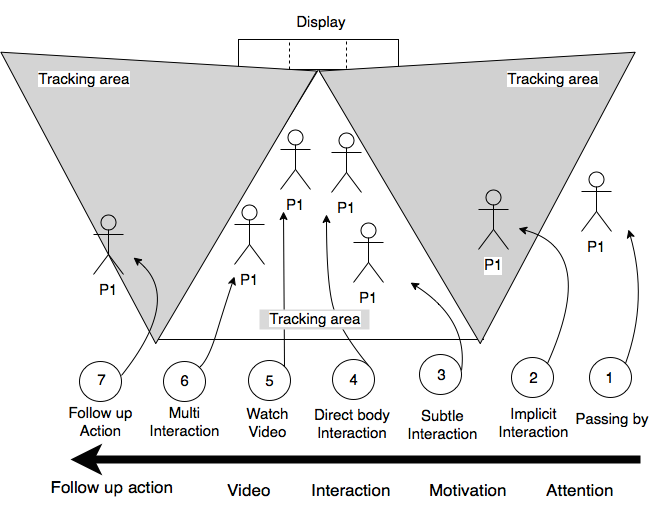
\includegraphics[width=0.85\textwidth,height=7.5cm]{Figures/9/enhanced_interaction_design}
    \caption{Extended Interaction design}%
    \label{fig:KinectExtended}%
\end{figure}




\section{Research question}
This experiment was conducted to find out that what are the major effects when the coverage area is expanded in both right and left side of the screen, compared to the previous body interation.

\begin{enumerate}
\item Would the attention level change?
\item Would the number of engaged passers-by increase?
\item Would the average engagement time rise?
\item Would there be any changes in number of Honeypot and landing effect?
\item What would be the passers-by behaviors to the display?
\end{enumerate}



\section{Study design}

\subsection{Location}
This experiment was conducted in the same location that was chosen in previous location, it was positioned in the same pathway of passers-by with the same height and screen brightness.  The surrounding of the display was also kept similar like the previous. 

\subsection{Duration}
This experiment was conducted only for three continues days at end of the week, Friday, Saturday, Sunday.

\subsection{Participants}
The participants were from Tourist information center; they were not informed that there is an interactive screen. Most of the participants were of old age, and the rest were middle aged and young aged participants. 

\subsection{Data gathering}
The bellow types of data were gathered during three days.

\begin{enumerate}
\item \textbf{On-Site Observation} \\
Observation periods were selected the same as the previous study, from 10:00 – 12:00 and the second was from 14:00 – 16:00, During these two time slots the bellow observations were made.

\begin{enumerate}
\item \textbf{Attention Level measurement} \\
Number of glances and number of ignores were counted by observing the passers-by from a fixed location, anyone who turned his/her face toward the display for less than 3 seconds were counted as glance, and those who had not turned their faces at all where selected as ignored. see the full report of glances in Appendix.
\hilight{fix the appendix}
%\ref{AppendixE}.1

\item \textbf{Passerby behavior} \\
The behaviors of the passers-by were observed by direct observation in onsite and also from the Camera depth recorded frames. From the observation two important effects were taken in consideration (honeypot and landing effect).


\end{enumerate}

\item \textbf{Colored-image recording} \\
A 2D colored image was taken per second from each of three cameras, and meanwhile were joint together side-by-side and after the image recording was done, in lab another post processing script was applied to integrate a static background using Adobe Photoshop application. To match the data logs and the image frames, each image name consisted time as (12.43.21.png).
Bellow three Kinect images stacked together, as can be seen that people's colored images was rendered on the images (1,2 and 3) these images are stacked together so that the transition of one person be smooth from one camera to the other.


\begin{minipage}{0.95\textwidth}
\begin{flushright}
\begin{figure}[H]
   \centering
    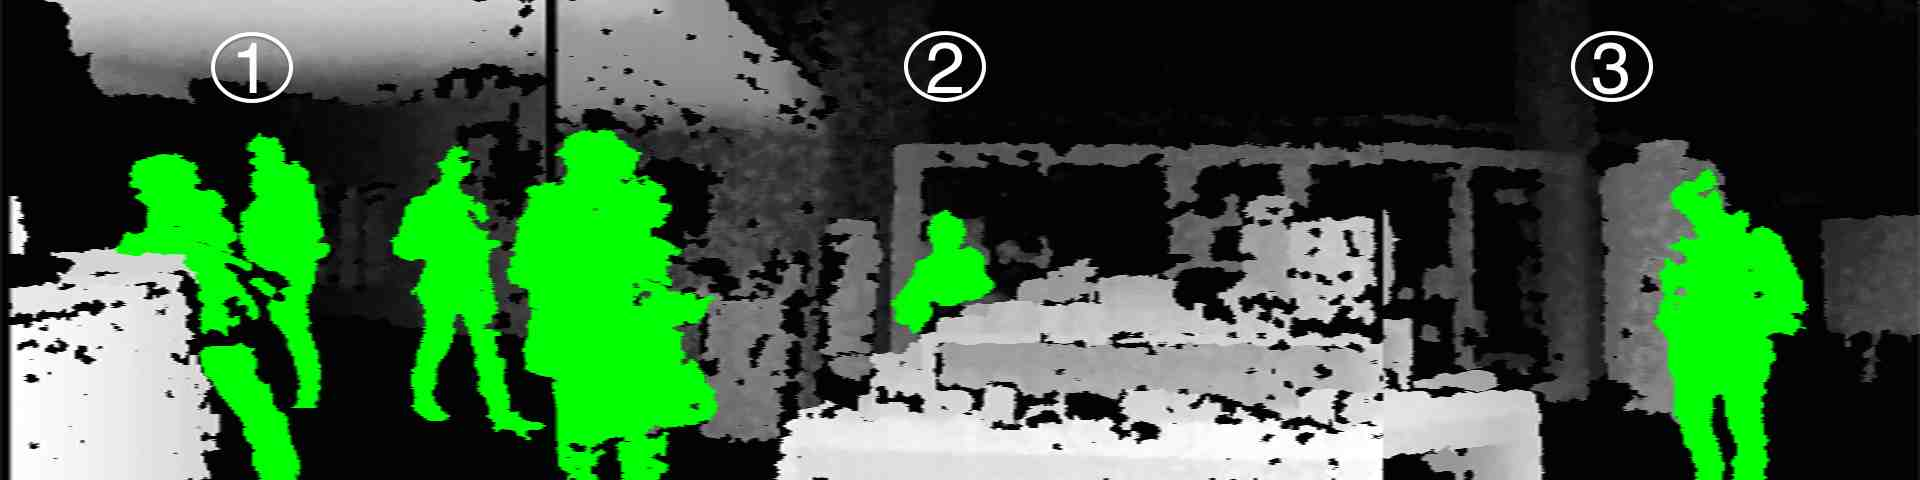
\includegraphics[width=\textwidth,height=40mm]{Figures/9/stacked_image}%
    \caption{Three Kinect images}%
    \label{fig:threekinectimages}%
\end{figure}
\end{flushright}
\end{minipage}


\end{enumerate}

\section{Findings and results}
This section first lists all the findings for enhanced version of advertisement then it compares it with the previous interactive advertisement.


\subsection{Attention Level measurements}
The bellow chart shows the number of glances and ignore for the following three days.

\begin{figure}[H]
    \centering
    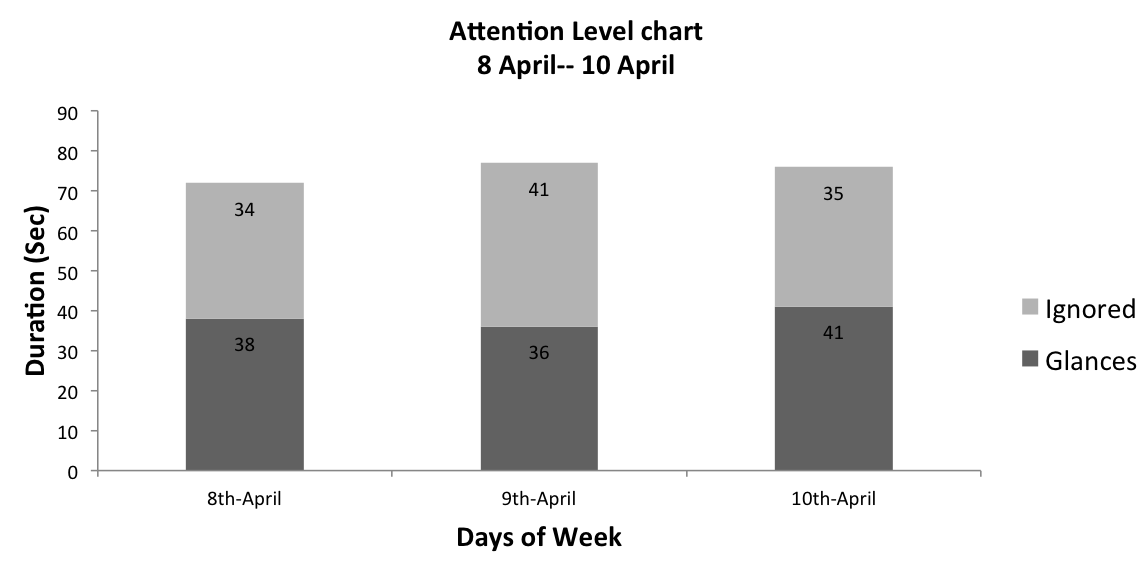
\includegraphics[width=110mm,height=55mm]{Figures/9/newbody_Inter_chart}%
    \caption{Attention level chart}%
    \label{fig:newbodyattentionlevelchart}%
\end{figure}


As can be seen from the above chart every day has almost similar number of glances and ignores and in average it makes about \%51 glances and \%49 ignores.


\begin{figure}[H]
    \centering
    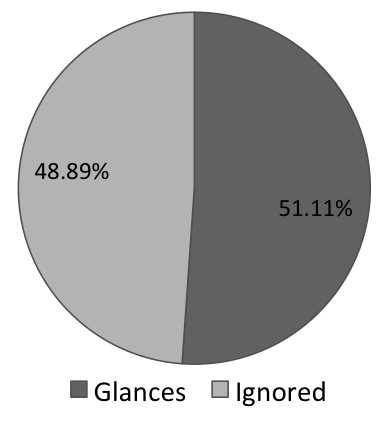
\includegraphics[width=60mm,height=55mm]{Figures/9/newbody_inter_percentage}
    \caption{Attention level percentage}%
    \label{fig:Nonattentionlevelpercentage}%
\end{figure}



\subsection{Engagement phases and time}
The engagement time for phases were measured from system logs and depth recording manually and in which people spent 16.10 seconds in average for the Attraction/Motivation phase some people took longer and some shorter, and some of them may have left without switching to the rest phases. 16.20 seconds in average was spent for interaction phase, which was different from person to person, and only 3.63 seconds in average was spent for video advertisement.

\begin{figure}[H]
    \centering
    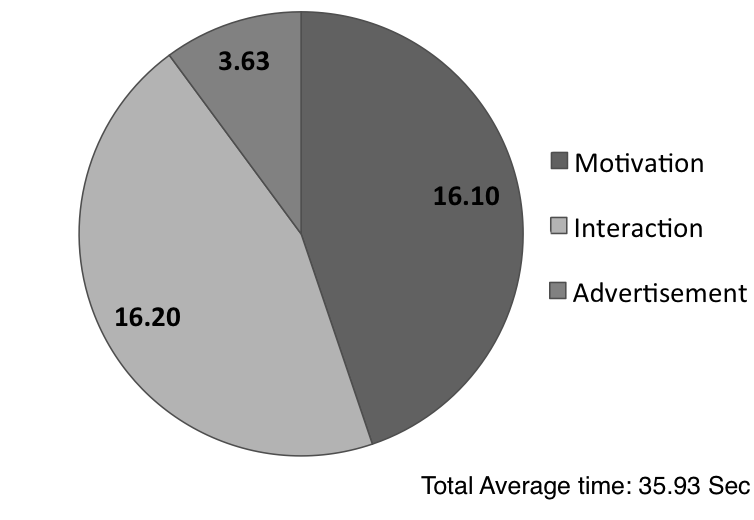
\includegraphics[width=90mm,height=60mm]{Figures/9/avg_phases}
    \caption{Average time for each phase}%
    \label{fig:newbodyaveragephases}%
\end{figure}

The entire average engagement duration for all these three phases together, was around 36 seconds.

\subsection{Number of engaged passers-by}
The entire three day’s recordings were manually analyzed frame by frame from which the number of passers-by were counted. The bellow chart shows all the count of passers-by and out of those the people who stood in front the screen for more than 3 seconds were flagged as an engaged passer-by. 

\begin{figure}[H]
    \centering
    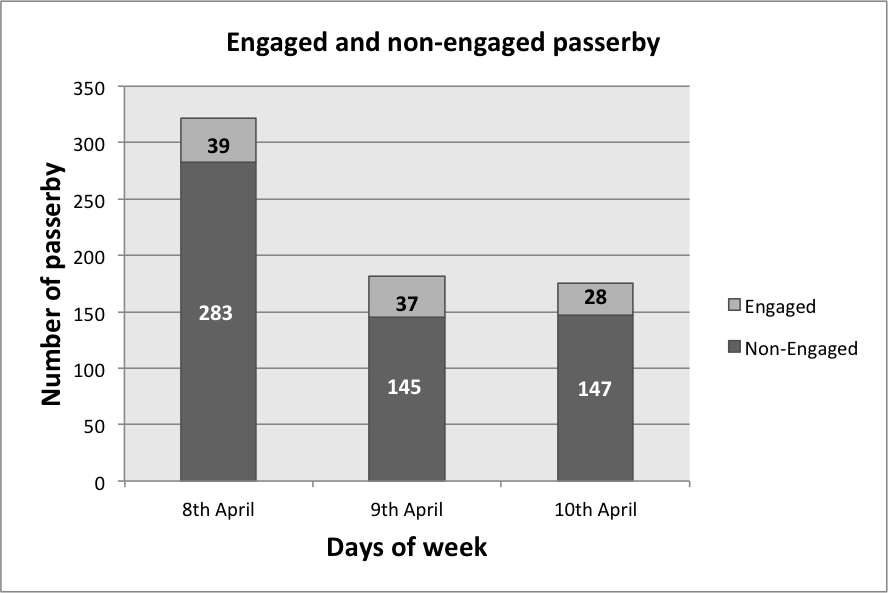
\includegraphics[width=0.9\textwidth,height=6.5cm]{Figures/9/newbody_inter_engage_day}
    \caption{Number of engaged passers-by}%
    \label{fig:newbodyengagedandengagedby}%
\end{figure}


From entire passers-by \%15.32 of them were engaged with the display and the rest might have only glanced or simply ignored as shown in the chart bellow.

\begin{figure}[H]
    \centering
    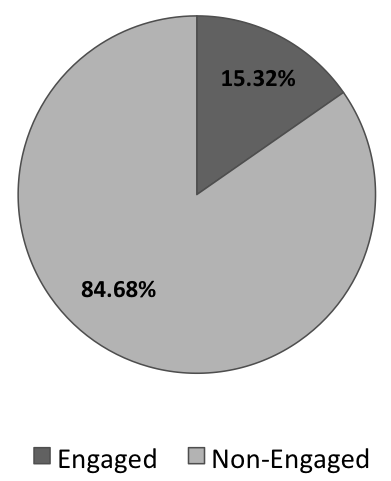
\includegraphics[width=60mm,height=60mm]{Figures/9/newbody_eng_percentage}
    \caption{Percentage of engaged and non-engaged passers-by}%
    \label{fig:newbodyengagedpasserbypercentage}%
\end{figure}


\newpage
\subsection{Landing and Honeypot effects}
Although the number of days were only for three days, but Landing effects \cite{LookingGlass} and Honeypot effects\cite{EnticingPeople} were observed for this type of technique and they were not as strong as in previous interaction technique. See the example frames bellow.


\begin{itemize}


\item Honeypot Effect:

\end{itemize}


\begin{wrapfigure}[22]{R}{0.55\textwidth}
  \vspace{-30pt}
  \begin{center}
    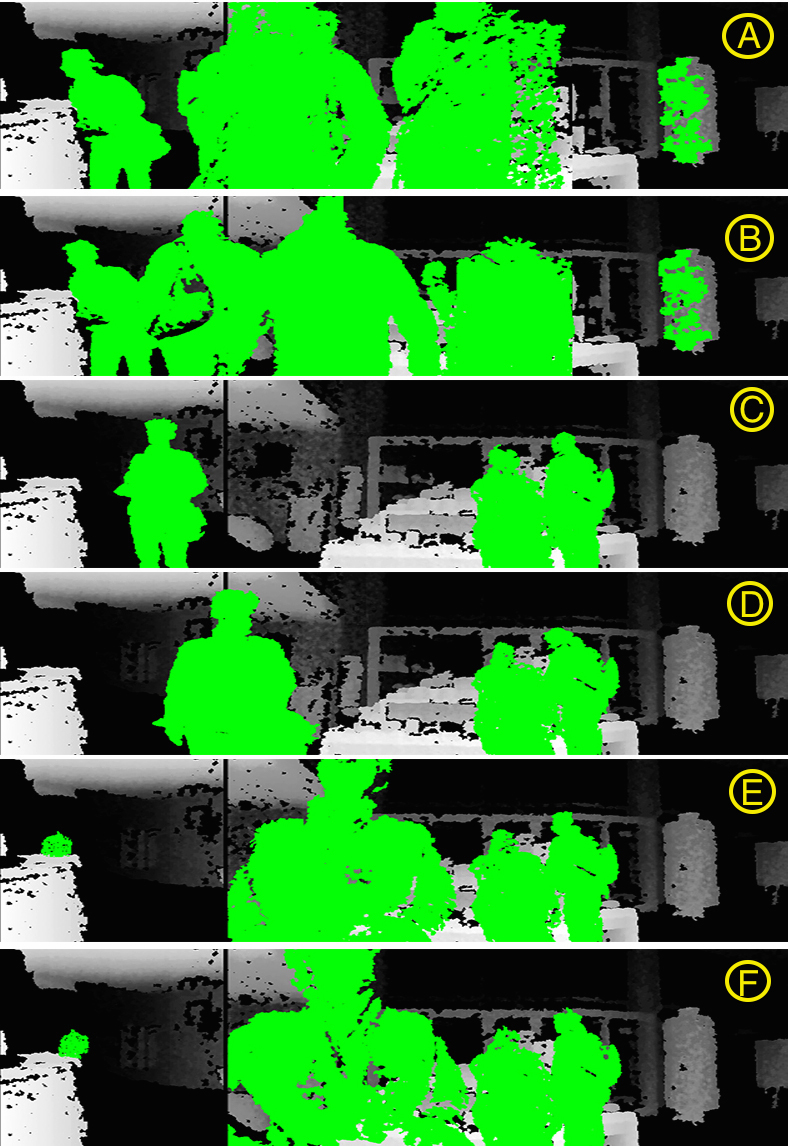
\includegraphics[width=0.55\textwidth,height=120mm]{Figures/9/effects/honeypot}
  \end{center}
  \vspace{-20pt}
  \caption{Honeypot effect}
  \vspace{-60pt}
\end{wrapfigure}
As can be seen from the picture in the right, which is composed of three kinect images that has covered right and left and the center of the display. 
In first frame (A) in the middle of the screen two persons are engaged and interacting for some time and a women at the left is busy with the help desk, but she is curious about the screen and has got attracted toward the screen, and she has looked many times in previous frames, in frame (B) the two guys leave the interaction and walk away from the screen and the application is left alone, and in frame (C) that women is left alone and is watching her self in the screen, and then approaches toward the screen in frame (D), she is near to the screen and I guess realizes that the screen is in fact interactive and in frame (E) she comes closer and starts actively interaction in frame (F). 
 



%\begin{figure}[H]
%    \centering
%    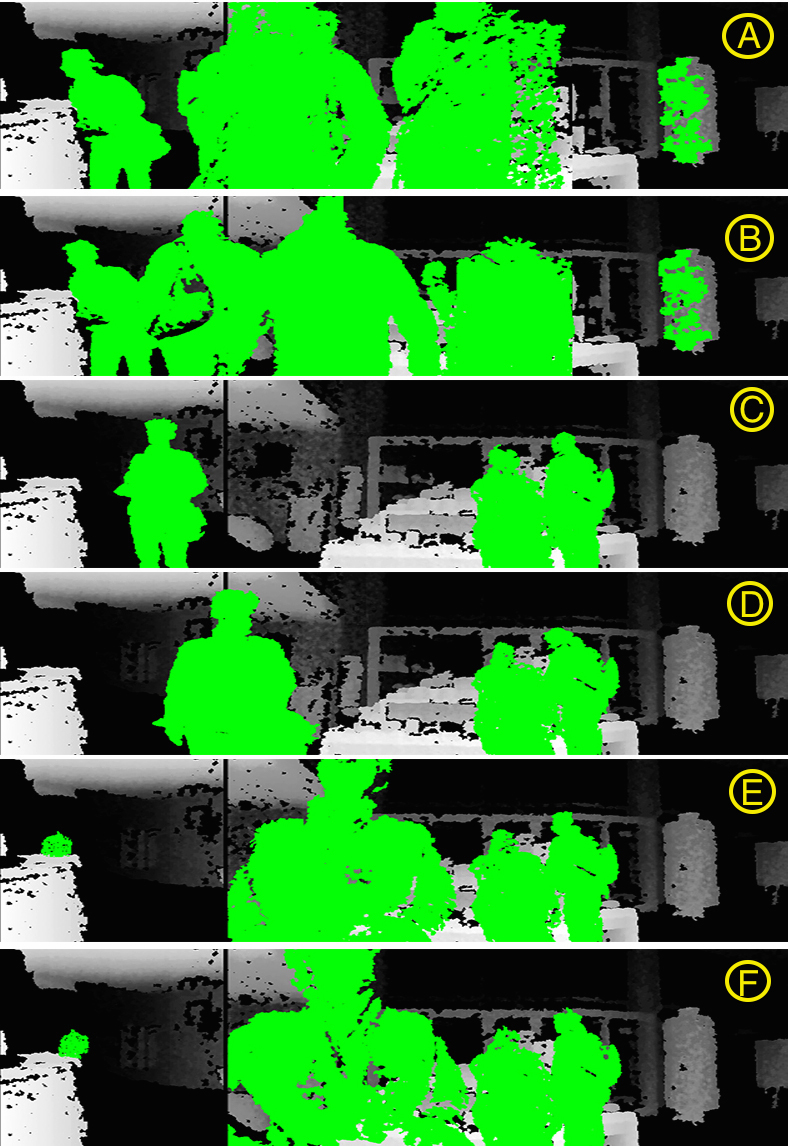
\includegraphics[width=0.6\textwidth,height=120mm]{Figures/9/effects/honeypot}
%    \caption{Honeypot effect}%
%    \label{fig:newbodyhoneypoteffect}%
%\end{figure}




\newpage
\begin{itemize}

\item Landing Effect:

\end{itemize}


\begin{wrapfigure}[30]{R}{0.55\textwidth}
  \vspace{-30pt}
  \begin{center}
    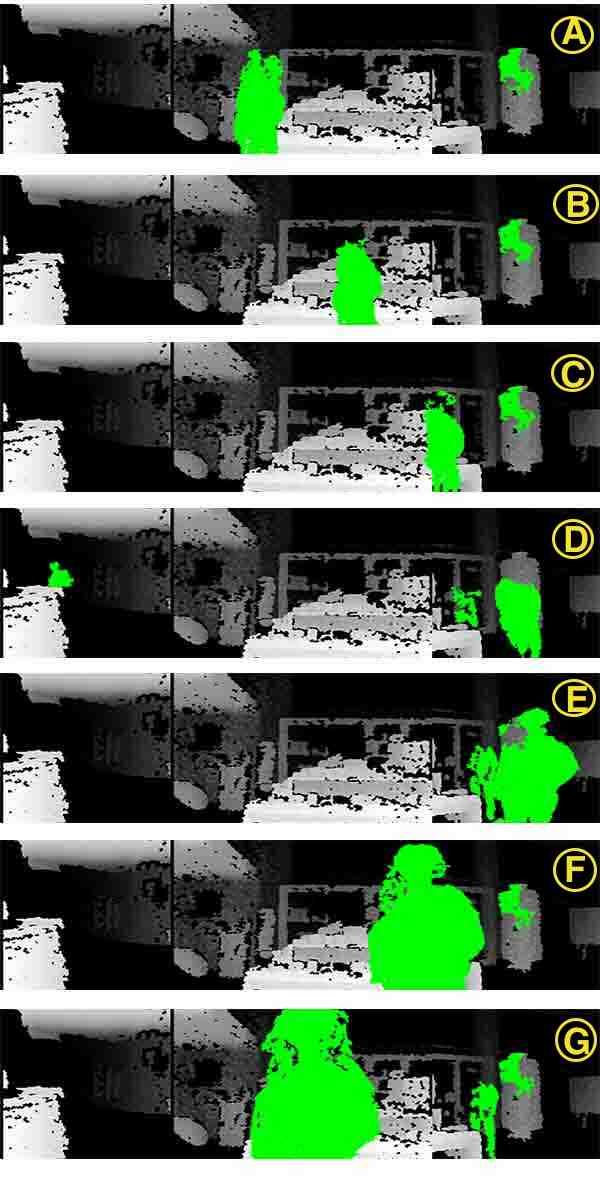
\includegraphics[width=0.55\textwidth,height=140mm]{Figures/9/effects/landing}
  \end{center}
  \vspace{-20pt}
  \caption{Landing effect}
  \vspace{-60pt}
\end{wrapfigure}
Few landing effects had also happened, which were similar to the previous experiment with one camera. The landing effect has happened differently like, some noticed the interactivity in the middle and stopped by the display, and some noticed the interactivity at the very corner of the display and then moved back toward. 
As can be seen in the picture in the right, there is a lady (the camera could not capture the entire body of her, maybe because of the sun light), the lady is passing by the screen from frame (A – D) continuously and notices the screen interactivity in frame (E) and stops at her position and when she realizes then she moves gets closer to the screen in frame (F) and reaches the middle of the screen at frame (G) and starts to explore the interaction and game.




\begin{itemize}

\item Numbers of Honeypot and Landing Effects: \\

\end{itemize}

The chart bellow shows the frequencies of landing and honeypot effects for three days. 


\begin{minipage}{\textwidth}
\begin{flushleft} 
\begin{table}[H]
\label{tab:landingandhonypot}
\resizebox{7cm}{1.3cm}{
\begin{tabular}{| l | c | c |}
\toprule
\tabhead{Days} & \tabhead{Landing effect} & \tabhead{Honeypot effect} \\
\midrule
8th April & 3 &  3 \\
9th April  & 2 &  5 \\
10th April  & 1 &  2 \\
\bottomrule
\end{tabular}
}
\end{table}
\end{flushleft} 
\end{minipage}


\subsection{Other observations}
%see Appendix Appendix \ref{AppendixE}.2
Beside the above behaviors there were other observations recorded too as they are listed bellow. 
\begin{itemize}

\item Calling Others: \\
When a person is engaged with the display and is more excited about it, the person will most likely call his / her friend or family to see and give it a try. 
\end{itemize}

\begin{wrapfigure}[30]{R}{0.5\textwidth}
  \vspace{-10pt}
  \begin{center}
    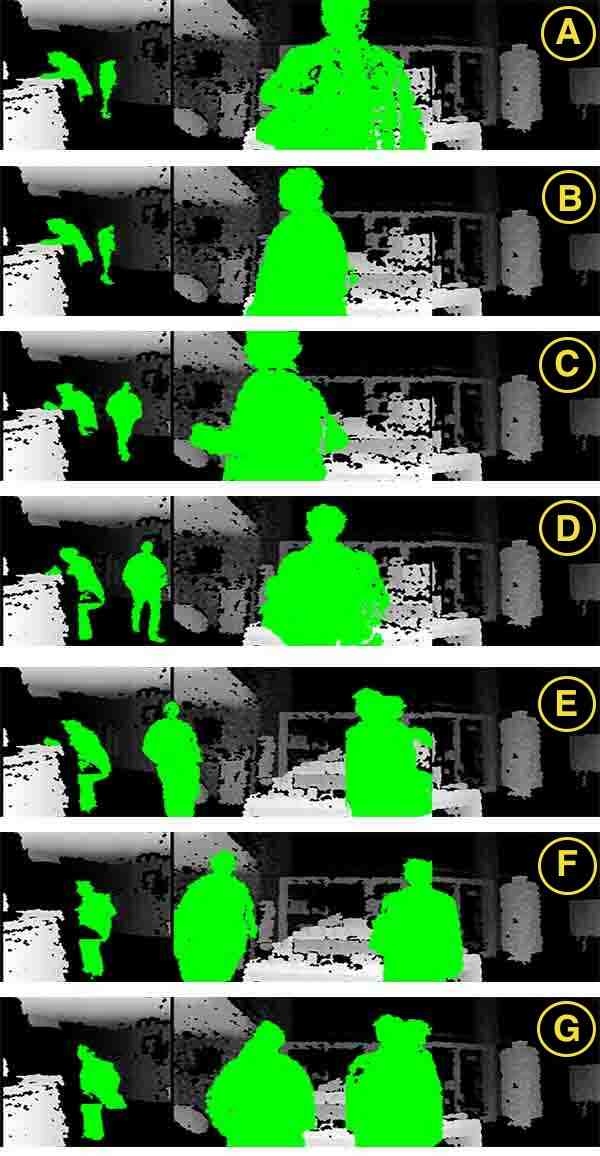
\includegraphics[width=0.50\textwidth,height=140mm]{Figures/9/effects/calling_others}
  \end{center}
  \vspace{-20pt}
  \caption{Calling others}
  \vspace{-20pt}
\end{wrapfigure}
Few of this calling effect have occurred in this enhanced version too, as you can see the picture in the right, in frame (A) a lady was engaged with the screen for a while and is standing in the middle of the screen, and then she calls his friend who is standing very far from the display and is busy with looking to some books, she turns her self toward her friend in frame (B) and seems to be talking to him in frame (C) and her friend leaves his work and starts to look at her in frame (C) and moves toward the screen in frame (D) while the lady is back busy with the screen, when her friend comes closer to the screen in frame (E) she gives a bit space for him to let him see by moving a bit back in frame (F), and finally her friend is also attracted and experiencing with the advertisement in frame (G).  
\break
\break
\break
\break
\break
\break
\break
\break



\begin{itemize}
\item Noticing Interactivity earlier:
\end{itemize}


\begin{wrapfigure}[20]{L}{0.48\textwidth}
  \vspace{-30pt}
  \begin{center}
    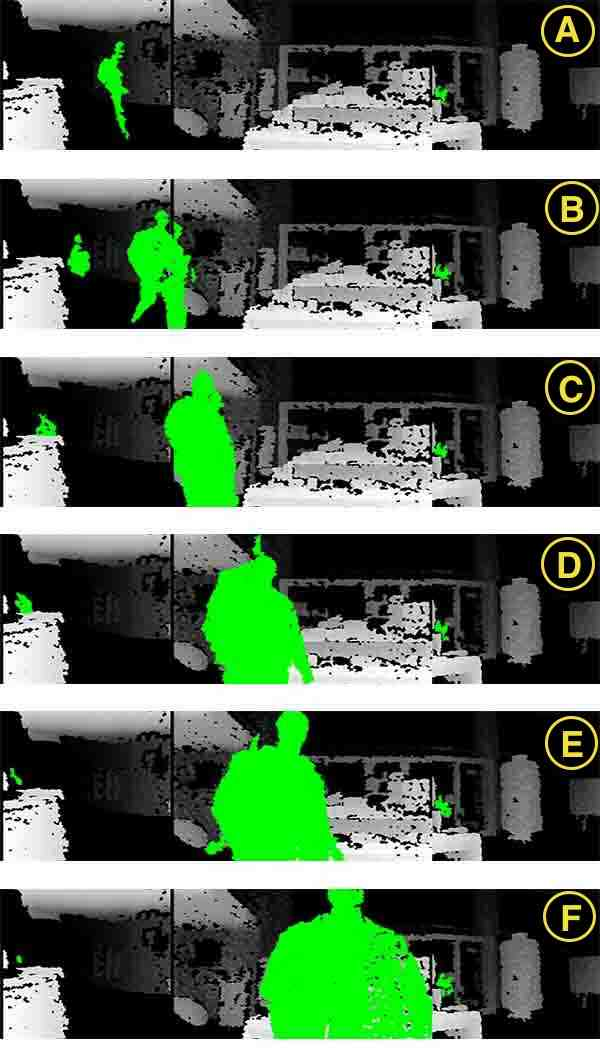
\includegraphics[width=0.45\textwidth,height=90mm]{Figures/9/effects/noticing_earlier}
  \end{center}
  \vspace{-20pt}
  \caption{Noticing interactivity earlier.}
  \vspace{-60pt}
\end{wrapfigure}
Passers-by also directly came from the corners of display without showing any landing effect toward the screen and started interacting, this effect might be because of when they were passing by the screen had noticed themselves on the screen from the first camera, which was faced toward the side of the display, so it is assumed that they understood the interactivity and then came in the center of the display and started interacting. As can be seen from the image at the left side, a person is walking by from the left side in frame (A) and continues his walking toward the screen and gets closer and closer toward the middle of the screen, he is not passing by the screen by he intentionally stops in the middle and starts interacting. 
\break


\begin{itemize}

\item Side interaction:

\end{itemize}


\begin{wrapfigure}[15]{R}{0.48\textwidth}
  \vspace{-30pt}
  \begin{center}
    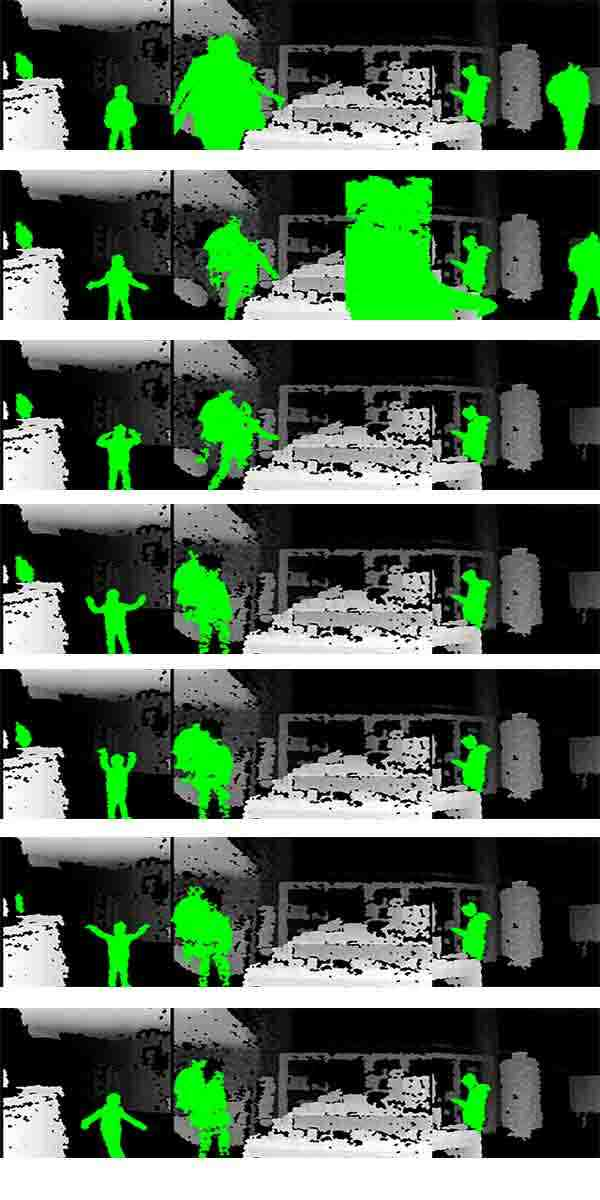
\includegraphics[width=0.48\textwidth,height=90mm]{Figures/9/effects/playing}
  \end{center}
  \vspace{-20pt}
  \caption{Side interaction}
  \vspace{-60pt}
\end{wrapfigure}
The integration of Kinect cameras at the side provided passers-by or people who were standing at the side of the display and did not or could not to come close to the screen, were still able to have some sort of bound or connection with the system, this feature provided a sense of safety comfort zone for them to stay back and still be able to interact passively. 

As can be seen in the picture in the right, there is a girl standing at the left side of the picture, she was standing with her parents in the information desk, and she recognizes herself in the screen and waves her hand first to see if it is actually her, and then starts to play with her silhouette on the screen and have fun.
\break
\break
\break
\break

\subsection{Comparison}
This section compares the results and findings of the enhanced version of advertisement version with the previous advertisement, which could only track the middle screen of the display. 

\begin{enumerate}
\item \textbf{Comparison of number of passers-by} \\

To be on safe side that the number of participants were statistically the same, the bellow computation has be applied on three similar days, which provides the base for further evaluations.

\begin{table}[H]
\caption{Number of people for three conditions}
\label{tab:newbodypasserbyofthreeweeks}
\centering
\resizebox{8cm}{1cm}{  
\begin{tabular}{| l | c | c | c |}
\toprule
\tabhead{Days} & \tabhead{Non-Interactive} & \tabhead{Body Interactive} & \tabhead{Enhanced body Interactive} \\
\midrule
\textbf{Day 1}  & 212 & 259 &  322 \\
\midrule
\textbf{Day 2}  & 209 & 216 &  182 \\
\midrule
\textbf{Day 3}  & 208 & 122 &  175 \\
\midrule
\textbf{Total}  & 629 & 597 &  679 \\
\bottomrule
\end{tabular}
}
\end{table}

ANOVA test revealed that there was no statistical significant different between the passers-by in each of the conditions (\emph{(F2,3)=0.1449, p >.05 (p=0.868)})



\item \textbf{Attention Level comparison}  \\
The number of glances and ignores for both body interaction and enhanced body interaction were collected as bellow.


\begin{table}[H]
\caption{Cross tabulation for each condition attention level}
\label{tab:newbodycrosstabulationweeks}
\centering
\resizebox{8cm}{1cm}{ 
\begin{tabular}{| l | c | c | c |}
\toprule
\tabhead{Method} & \tabhead{Glanced (\%)} & \tabhead{Ignored} & \tabhead{Total } \\
\midrule
\textbf{Non-interactive}     & 111(\%28.83)   &   274      &   385\\
\midrule
\textbf{Body Interactive}     & 106 (\%41.40)   &   150      &   256\\
\midrule
\textbf{Enhanced body Interactive }   & 115 (\%51.11)  &   110      &   225\\
\midrule
\textbf{Total }         		 & 332            &   534      &   866\\
\bottomrule
\end{tabular}
}
\end{table}


As can be seen the enhanced body interactive advertisement has a higher percentage about \%51 of the glances compared to the old body interactive advertisement, this means that there is a rise of \%10 increase. To test if these are statistically significant different, the Chi-square test was applied on them and revealed ${\chi}^2$\emph{(1, N=481)=4.5413, p < .05 (p=.033086)} that they are statistically different and the enhanced body attraction technique does have higher effect on the attention level. 

The non-interactive advertisement was about \%28 percentage in attracting attention, but the enhanced version had about \%23 higher attention level than non-interactive, Chi-square reveals ${\chi}^2$\emph{(1, N=610)=30.2247, p < .001 (p=.0)}, which strongly suggests that the enhanced version has dramatically increased the attention level than the non-interactive one.


\item \textbf{Engaged and Non-engaged passers-by} \\
The numbers of engaged and non-engaged were recorded for all three conditions as bellow.

\begin{table}[H]
\caption{Number of engaged passers-by in three weeks}
\label{tab:engagedofthreeweeks}
\centering
\resizebox{8cm}{1cm}{  
\begin{tabular}{| l | c | c | c |}
\toprule
\tabhead{Days} & \tabhead{Non-Interactive} & \tabhead{Body Interactive} & \tabhead{Enhanced body Interactive } \\
\midrule
\textbf{Day 1}  & 15 & 26 &  39 \\
\midrule
\textbf{Day 2}  & 15 & 20 &  37 \\
\midrule
\textbf{Day 3}  & 15 & 23 &  28 \\
\midrule
\textbf{Total}  & 45 & 69 &  104\\
\bottomrule
\end{tabular}
}
\end{table}


ANOVA reveals that there was statistical difference between these conditions, (\emph{(F2,3)=20.3154, p <.05 (p=0.0021)}), and to confirm that which of the pairs were different significantly, I run Post-Hoc Tukey’s HSD test as bellow.


\begin{table}[H]
\caption{Post-Hoc Tukey’s HSD}
\label{tab:engage-non-posthoctukey}
\centering
\resizebox{0.9\textwidth}{!}{  
\begin{tabular}{| l | c | c | c |}
\toprule
\tabhead{Methods} & \tabhead{Tukey HSD Q statistic} & \tabhead{Tukey HSD p-value} & \tabhead{Tukey HSD inferfence} \\
\midrule
\textbf{A vs B}  & 3.6459 & 0.0920761 &  insignificant  \\
\midrule
\textbf{A vs C}  & 8.9627 & 0.0017440 &  ** p<0.01 \\
\midrule
\textbf{B vs C}  & 5.3169 & 0.0218582 &  * p<0.05 \\

\bottomrule
\end{tabular}
}
\end{table}


Group A, B and C refers to (Non-interactive, body interactive and enhanced body interactive) advertisement accordingly. Post-hoc Tukey computed the critical value(Studentized Range Q statistic) for A and C as, ${Q}_{critical}^{\alpha=0.01,k=6}$ = 6.3250 and another critical value for B and C as, ${Q}_{critical}^{\alpha=0.05,k=6}$ = 4.3341 and the significance can be determined if each pair’s critical value(Tukey HSD Q statistic) is bigger than Studentized Range Q statistic. ${Q}_{j}^{i }$ > ${Q}_{critical}$, and the strength of difference is determined by the \emph{P} value as shown above. 

From the diagram above it is very clear that non-interactive with body interactive is insignificant because their critical value is smaller than 4.3341 and p > 0.05, the result was significant in the previous chapter because of five days together but became insignificant with little number of days. On the other hand, the non-interactive with enhanced body interactive is strongly significant because their critical value is bigger than 6.3250 with p < 0.01, the result of enhanced body compared to body interactive is also significant with p<0.05. As a result the enhance body interactive has strongly increased the number of engaged passers-by compared to non-interactive advertisement, and the effect size between them are measured as bellow.


To find out how big is the difference between number of engaged passers-by in non-interactive and enhanced body interactive conditions, the eta squared(${\eta}^2$), which is an effect size index for \emph{ANOVA}, in which the $SS_{effect}$ (sum of squared) between conditions is divided by $SS_{total}$  (sum of squared) total as bellow calculated by online tool \emph{Easycalculator}\footnote{easycalculator: \url{https://www.easycalculation.com/statistics/eta-square-calculator.php}, last accessed 15 jun 2016}.
\[
{\eta}^2 = \frac{{SS}_{effect}}{{SS}_{total}} = \frac{580.1687}{648.8354} = 0.8942\approx 0.89
\]

The 0.89 means that \%89 of total variance is accounted for by the conditions (enhanced body interactive, non-interactive) effect.



\item \textbf{Landing effect comparison}\\
The landing effects were recorded for non-interactive, body interactive and enhanced body interactive in bellow table.

\begin{table}[H]
\caption{Cross tabulation for each condition Landing effect }
\label{tab:newbodylandingeffect}
\centering
\resizebox{8cm}{1cm}{  
\begin{tabular}{| l | c | c | c |}
\toprule
\tabhead{Method} & \tabhead{Non-Interactive} & \tabhead{Body Interactive} & \tabhead{Enhanced body Interactive } \\
\midrule
\textbf{Day 1}    & 2    &   2      &   1\\
\midrule
\textbf{Day 2 }   & 0    &   2      &   2\\
\midrule
\textbf{Day 3}    & 1    &   3      &   3\\
\bottomrule
\end{tabular}
}
\end{table}
After conducting ANOVA test, it states that there is no significant different between three days for all of the conditions, 
(\emph{(F2,3)=1.857, p >.05 (p=0.236)}). 


\item \textbf{Honeypot effect comparison}\\
Honeypot effects were also gathered from those days as bellow in table.

\begin{table}[H]
\caption{Cross tabulation for each condition Honeypot effect }
\label{tab:newbodyhoneypoteffect}
\centering
\resizebox{8cm}{1cm}{  
\begin{tabular}{| l | c | c | c |}
\toprule
\tabhead{Days} & \tabhead{Non-Interactive} & \tabhead{Body Interactive} & \tabhead{Enhanced body Interactive } \\
\midrule
\textbf{Day 1}    & 2    &   2      &   3\\
\midrule
\textbf{Day 2 }   & 2    &   5      &   5\\
\midrule
\textbf{Day 3}    & 1    &   3      &   2\\
\bottomrule
\end{tabular}
}
\end{table}

ANOVA reveals that there is also no statistical difference between these conditions. \\
(\emph{(F2,3)=1.667, p >.05 (p=0.266)})


\end{enumerate}


\newpage
\section{Discussions}
The increase in attention level, which was higher than old body advertisement version could have many reasons, (1)\emph{Wide angle tracking}, the wide angle of display tracking, in which participants could see themselves from different angles (left, center and right) if they had missed the left, there was still chance to see the center or vice versa, and (2) \emph{Exposure time}, the time passers-by were exposed to their silhouette in three cameras facing (left, center, right), was longer than exposure time with only one camera, normally it takes around 1.2 seconds to understand interactivity with silhouette with large screen that is in front of passers-by \cite{ LookingGlass}.

Honeypot effect in the previous body interaction experiment and in this experiment did not seemed to be more strong, there could be many reasons for this, (1) \emph{Environment}, the display is situated in a touristic place, where people do not stay longer than staying in restaurant or some other gatherings, people move in and out often times, (2) \emph{unfamiliarity}, people are not familiar with each other to wait or come near to the shoulder of other person to look what is going on, therefor they tend to ignore, (3) \emph{Personal interaction}, the interaction seemed more personal and single user,  and was not vast to be observed by others quickly, (4) \emph{display size}, screen size was also small and passers-by might have not noticed the interactions of people.

As mentioned before, landing effect happens, when the user notices interactivity after he passes by the screen, but in this enhanced version few honeypot effects happened, one of the reasons could be that, when the passer-by is walking from a far side of the display, he is noticing the interactivity before hand because he can see himself in the screen, and when he reaches near to the screen, he is aware of the interactivity for sure and would not perform landing, but by that time he would have two options (a) start interacting, or (b) ignore the interaction and pass by the screen.

\section{Conclusion}
In conclusion, this enhanced body interactive version performed significantly better than body interactive technique, it has increased the attention level of passers-by and dramatically raised the number of engaged people in front of display, but the number of landing and honeypot effects were not significant compared to body interactive. 

In enhance version, the number of glances was \%51 against the number of ignores, it was very effective in attention level than other two conditions (non-interactive and body interactive), because the number of glances was almost double than non-interactive and \%10 increase than body interactive. The findings show that for a display positioned in a sideway, this technique can increase the attention level significantly than non-interactive display.

The enhanced version also increased the number of engaged people up to\%15 of whole passers-by during three days, which the body interactive could not achieve in five days (\%12) and the findings state that the enhanced version significantly engaged people than body interactive, but the significance was not as strong as compared to non-interactive (\%7), which was above the double of percentage of engaged. 

The above percentages might would have increased if the silhouette color was not the same for all passers-by, various silhouette color has an effect on the attention level and the motivation on passers-by, it would be very effective if this problem gets fixed in future. 




